\setcounter{subsection}{16-1}
\subsection{The Subspace Topology}

\exercise{1}{
  Show that if $Y$ is a subspace of $X$ and $A$ is a subspace of $Y$, then the topology $A$ inherits as a subspace of $Y$ is the same as the topology it inherits as a subspace of $X$.
}
\sol{
  \dwhitman

  \qproof{
    Let $\cT$ be the topology on $X$ and  $\cT_Y$ be the subspace topology that $Y$ inherits from $X$.
    Also let $\cT_A$ and $\cT_A'$ be the topologies that $A$ inherits as a subspace of $Y$ and $X$, respectively.
    Therefore we must show that $\cT_A = \cT_A'$.
    Now, by definition of subspace topologies we have that,
    \ali{
      \cT_Y &= \braces{Y \cap U \where U \in \cT} &
      \cT_A &= \braces{A \cap U \where U \in \cT_Y} &
      \cT_A' &= \braces{A \cap U \where U \in \cT} \,.
    }
    Now suppose that $W \in \cT_A$ so that $W = A \cap V$ for some $V \in \cT_Y$.
    Then we have that $V = Y \cap U$ for some $U \in \cT$, and hence
    \gath{
      W = A \cap V = A \cap (Y \cap U) = (A \cap Y) \cap U = A \cap U
    }
    since we have that $A \cap Y = A$ since $A \ss Y$.
    Since $U \in \cT$ this clearly shows that $W \in \cT_A'$ so that $\cT_A \ss \cT_A'$ since $W$ was arbitrary.

    Then, for any $W \in \cT_A'$, we have that $W = A \cap U$ for some $U \in \cT$.
    Let $V = Y \cap U$ so that clearly $V \in \cT_Y$.
    Then as before we have that $A = A \cap Y$ since $A \ss Y$ so that
    \gath{
      W = A \cap U = (A \cap Y) \cap U = A \cap (Y \cap U) = A \cap V \,,
    }
    and thus $W \in \cT_A$ since $V \in \cT_Y$.
    Since $W$ was arbitrary this shows that $\cT_A' \ss \cT_A$, which completes the proof that $\cT_A = \cT_A'$.
  }
}

\exercise{2}{
  If $\cT$ and $\cT'$ are topologies on $X$ and $\cT'$ is strictly finer than $\cT$, what can you say about the corresponding subspace topologies on the subset $Y$ of $X$?
}
\sol{
  \dwhitman

  Let $\cT_Y$ and $\cT_Y'$ be the subspace topologies on $Y$ corresponding to $\cT$ and $\cT'$, respectively.
  We claim that $\cT_Y$ is finer than $\cT_Y$ but not necessarily strictly finer.
  \qproof{
    First, we have that
    \ali{
      \cT_Y &= \braces{Y \cap U \where U \in \cT} &
      \cT_Y' &= \braces{Y \cap U \where U \in \cT'}
    }
    by the definition of subspace topologies.
    So for any $V \in \cT_Y$ we have that $V = Y \cap U$ where $U \in \cT$.
    Then also $U \in \cT'$ since $\cT'$ is finer than $\cT$.
    This shows that $V \in \cT_Y'$ since $V = Y \cap U$ where $U \in \cT'$.
    Hence $\cT_Y'$ is finer than $\cT_Y$ since $V$ was arbitrary.

    To show that it is not necessarily strictly finer, consider the sets $X = \braces{a,b,c}$ and $Y = \braces{a,b}$ so that clearly $Y \ss X$.
    Consider also the topologies
    \ali{
      \cT &= \braces{\es, X, \braces{a,b}} &
      \cT' &= \braces{\es, X, \braces{a,b}, \braces{c}} 
    }
    on $X$ so that clearly $\cT'$ is strictly finer than $\cT$.
    This results in the subspace topologies
    \ali{
      \cT_Y &= \braces{\es, Y} &
      \cT_Y' &= \braces{\es, Y} \,,
    }
    which are clearly the same so that $\cT_Y'$ is not strictly finer than $\cT_Y'$, noting that it is technically still finer.
    However, if we instead have the topologies
    \ali{
      \cT &= \braces{\es, X, \braces{a,b}} &
      \cT' &= \braces{\es, X, \braces{a,b}, \braces{b}} 
    }
    then 
    \ali{
      \cT_Y &= \braces{\es, Y} &
      \cT_Y' &= \braces{\es, Y, \braces{b}}
    }
    so that $\cT_Y'$ \emph{is} strictly finer than $\cT_Y$.
    Thus we can say nothing about the strictness of relation of the subspace topologies.
  }
}

\def\oh{\tfrac{1}{2}}
\exercise{3}{
  Consider the set $Y = [-1, 1]$ as a subspace of $\reals$.
  Which of the following sets are open in $Y$?
  Which are open in $\reals$?
  \ali{
    A &= \braces{x \where \oh < \abs{x} < 1}, \\
    B &= \braces{x \where \oh < \abs{x} \leq 1}, \\
    C &= \braces{x \where \oh \leq \abs{x} < 1}, \\
    D &= \braces{x \where \oh \leq \abs{x} \leq 1}, \\
    E &= \braces{x \where 0 < \abs{x} < 1 \text{ and } 1/x \notin \pints}.
  }
}
\sol{
  \dwhitman
  
  \begin{lem}\label{lem:subset:abs}
    If $a,b \in \reals$ such that $0 \leq a < b$ then the following are true:
    \ali{
      \braces{x \in \reals \where a < \abs{x} < b} &= (-b, -a) \cup (a, b) &
      \braces{x \in \reals \where a \leq \abs{x} \leq b} &= [-b, -a] \cup [a, b] \\
      \braces{x \in \reals \where a \leq \abs{x} < b} &= \opcl{-b, -a} \cup \clop{a, b} &
      \braces{x \in \reals \where a < \abs{x} \leq b} &= \clop{-b, -a} \cup \opcl{a, b} \,.
    }
  \end{lem}
  \qproof{
    We prove only the first of these as the rest follow from nearly identical arguments.
    Let $A = \braces{x \in \reals \where a < \abs{x} < b}$ and $B = (-b, -a) \cup (a, b)$ so that we must show that $A = B$.

    So consider $x \in A$ so that $a < \abs{x} < b$.
    If $x \geq 0$ then $\abs{x} = x$ so that $a < x < b$ and hence $x \in (a,b)$.
    If $x < 0$ then $\abs{x} = -x$ so that $a < -x < b$, and thus $-a > x > -b$ so that $x \in (-b, -a)$.
    Thus in either case $x \in B$ so that $A \ss B$.

    Now let $x \in B$ so that either $x \in (-b,-a)$ or $x \in (a,b)$.
    In the former case we have that $x < -a \leq 0$ since $a \geq 0$ so that $\abs{x} = -x$ and therefore
    \gath{
      x \in (-b, -a) \imp -b < x < -a \imp b > -x = \abs{x} > a \imp x \in A \,.
    }
    In the  latter case we have that $x > a \geq 0$ so that $\abs{x} = x$ and therefore
    \gath{
      x \in (a, b) \imp a < x = \abs{x} < b \imp x \in A \,.
    }
    This shows that $B \ss A$ since $x$ was arbitrary, and thus $A = B$ as desired.
  }

  \begin{lem}\label{lem:subset:open}
    Suppose that $X$ is a topological space and $Y \ss X$ with the subspace topology.
    Then, if a set $U \ss Y$ is open in $X$, then it is also open in $Y$.
  \end{lem}
  \qproof{
    So suppose that $U \ss Y$ is open in $X$.
    Then we have that $Y \cap U = U$ is also open in $Y$ by the definition of the subspace topology.
  }

  \mainprob

  First we claim that $A$ is open in both $\reals$ and $Y$.
  \qproof{
    We have from Lemma~\ref{lem:subset:abs} that $A = (-1, -\oh) \cup (\oh, 1)$ which is clearly the union of basis elements so that $A$ is open in $\reals$.
    We also have that $A \ss Y$ so that $A$ is open in $Y$ by Lemma~\ref{lem:subset:open} since it is open in $\reals$.
  }

  Next we claim that $B$ is open in $Y$ but not in $\reals$.
  \qproof{
    By Lemmma~\ref{lem:subset:abs} we have that $B = \clop{-1, -\oh} \cup \opcl{\oh, 1}$.
    First, consider the sets $(-2,-\oh)$ and $(\oh,2)$, which are clearly both basis elements and therefore open in $\reals$.
    We then have that $(-2,-\oh) \cap Y = \clop{-1,-\oh}$ and $(\oh,2) \cap Y = \opcl{\oh, 1}$ so that these sets are open in $Y$ by the definition of the subspace topology.
    Clearly then their union $B = \clop{-1, -\oh} \cup \opcl{\oh, 1}$ is then also open in $Y$.

    It is also easy to see that $B$ is not open in $\reals$.
    For example, $-1 \in B$ but for any basis element $B' = (a,b)$ containing $-1$ we have that $a < -1 < b$ so that $a < (a-1)/2 < -1 < b$ and hence $(a-1)/2 \in B'$.
    Clearly though $(a-1)/2 \notin B$ so that $B'$ cannot be a subset of $B$.
    Thus suffices to show that $B$ is not open by the definition of the topology of $\reals$ generated by its basis.
  }

  We claim that $C$ is open neither in $\reals$ nor $Y$.
  \qproof{
    By Lemmma~\ref{lem:subset:abs} we have that $C = \opcl{-1,-\oh} \cup \clop{\oh, 1}$.
    If $\cB$ is the standard basis on $\reals$, then, by Lemma~16.1, the set $\cB_Y = \braces{B \cap Y \where B \in \cB}$ is a basis for the subspace $Y$.
    So consider the point $x = \oh$ and any basis element $B_Y \in \cB_Y$ containing $x$.
    Then we have that $B_Y = Y \cap B_X$ for some basis element $B_X = (a,b)$ in $\cB$, and thus $a < x < b$ since $x \in B_X$.
    Let $a' = \max(a, -\oh)$ and set $y = (a'+x)/2$ so that
    \gath{
      a \leq a' < (a'+x)/2 = y < x < b \,,
    }
    and hence $y \in (a,b) = B_X$.
    Also we have
    \gath{
      -1 < -\oh \leq a' < (a'+x)/2 = y < x = \oh < 1
    }
    so that $y \in [-1,1] = Y$.
    Therefore $y \in Y \cap B_X = B_Y$.
    However, since $-\oh < y < \oh$, clearly $y \notin C$ so that $B_Y$ cannot be a subset of $C$.
    Since the basis element $B_Y \in \cB_Y$ was arbitrary, this suffices to show that $C$ cannot be open in $Y$ since $\cB_Y$ is a basis.
    Since also clearly $C \ss Y$, it follows from the contrapositive of Lemma~\ref{lem:subset:open} that $C$ is not open in $\reals$ either.
  }

  Next we claim that $D$ is also not open in $\reals$ or $Y$.
  \qproof{
    This follows from basically the same argument as the previous proof, again using the point $x = \oh$ to show that any basis element of $Y$ that contains $x$ cannot be a subset of $D$.
  }

  Lastly, we claim that $E$ is open in both $\reals$ and $Y$.
  \qproof{
    First, it is trivial to show that
    \gath{
      E = \braces{x \in \reals \where 0 < \abs{x} < 1} - K = \squares{(-1,0) \cup (0,1)} - K \,,
    }
    where we have used Lemma~\ref{lem:subset:abs}.
    Now consider any $x \in E$ so that $x \in (-1,0) \cup (0,1)$ and $x \notin K$.
    If $x \in (-1,0)$ then clearly the basis element $(-1,0)$ contains $x$ and is a subset of $E$ since $(-1,0) \cap K = \es$.

    On the other hand, if $x \in (0,1)$ then $x \notin K$ so that $1/x \notin \pints$.
    From this it follows from Exercise~4.9b that there is exactly one positive integer $n$ such that $n < 1/x < n+1$.
    We then have that $1/(n+1) < x < 1/n$.
    So let $B = (1/(n+1), 1/n)$ so that clearly $x \in B$, $B \cap K = \es$, and $B$ is a basis element of the standard topology on $\reals$.
    Since $B \cap K = \es$ and clearly $0 < 1/(n+1) < 1/n \leq 1$, it also follows that $B \ss E$.

    Hence in either case there is a basis element of $\reals$ that contains $x$ and is a subset of $E$.
    This suffices to show that $E$ is open in $\reals$.
    Since clearly $E \ss Y$, we also clearly have that $E$ is open in $Y$ by Lemma~\ref{lem:subset:open}.
  }
}

\exercise{4}{
  A map $f: X \to Y$ is said to be an \boldit{open map} if for every open set $U$ of $X$, the set $f(U)$ is open in $Y$.
  Show that $\pi_1 : X \times Y \to X$ and $\pi_2 : X \times Y \to Y$ are open maps.
}
\sol{
  \dwhitman

  \qproof{
    Suppose that $U$ is an open subset of $X \times Y$.
    Consider any $x \in \pi_1(U)$ so that there is a $y \in Y$ such that $(x,y) \in U$.
    Then there is a basis element $A \times B$ of the product topology on $X \times Y$ where $(x,y) \in A \times B \ss U$.
    Then $A$ and $B$ are open sets of $X$ and $Y$, respectively, since $A \times B$ is a basis element of the product topology.
    Clearly we have that $x \in A$ since $(x,y) \in A \times B$.
    Now, for any $x' \in A$, we have that $(x',y) \in A \times B$ so that $(x',y) \in U$.
    Hence $x' = \pi_1(x',y) \in \pi_1(U)$, which shows that $A \ss \pi_1(U)$ since $x'$ was arbitrary.
    Then, since $A$ is an open subset of $X$, there is a basis element $A'$ where $x \in A' \ss A \ss \pi_1(U)$.
    This suffices to show that $\pi_1(U)$ is an open subset of $X$ since $x$ was arbitrary.
    An analogous argument shows that $\pi_2$ is also an open map.
  }
}

\exercise{5}{
  Let $X$ and $X'$ denote a single set in the topologies $\cT$ and $\cT'$, respectively; let $Y$ and $Y'$ denote a single set in the topologies $\cU$ and $\cU'$, respectively.
  Assume these sets are nonempty.
  \eparts{
  \item Show that if $\cT' \sps \cT$ and $\cU' \sps \cU$, then the product topology on $X' \times Y'$ is finer than the product topology on $X \times Y$.
  \item Does the converse of (a) hold? Justify your answer.
  }
}
\sol{
  \dwhitman

  In what follows let $\cT_p'$ and $\cT_p$ denote the product topologies on $X' \times Y'$ and $X \times Y$, respectively.
  
  (a)
  \qproof{
    Consider any $W \in \cT_p$ and any $(x,y) \in W$, noting that obviously $W \ss X \times Y$.
    Then there is a basis element $U \times V$ of $\cT_p$ such that $(x,y) \in U \times V$ and $U \times V \ss W$.
    By the definition of the product topology, we have that $U$ and $V$ are open sets in $\cT$ and $\cU$, respectively.
    Then we also have that $U \in \cT'$ and $V \in \cU'$ since $\cT \ss \cT'$ and $\cU \ss \cU'$.
    Hence $U \times V$ is also a basis element of $\cT_p'$.
    Since we know that $(x,y) \in U \times V$, $U \times V \ss W$, and $(x,y) \in W$ was arbitrary, this suffices to show that $W$ is an open subset of $X' \times Y'$ and hence $W \in \cT_p'$.
    This in turn shows that $\cT_p \ss \cT_p'$ since $W$ was arbitrary.
  }

  (b) We claim that the converse does not always hold.
  \qproof{
    As a counterexample consider $A = \braces{a, b, c, d}$ so that clearly
    \ali{
      \cT' &= \braces{\es, A, \braces{a,b}, \braces{c,d}} \\
      \cT &= \braces{\es, A, \braces{a,b}, \braces{c,d}, \braces{c}, \braces{d}, \braces{a,b,c}, \braces{a,b,d}} 
    }
    are topologies on $A$.
    Clearly also $\cT'$ is not finer than $\cT$.
    Similarly let $B = \braces{1, 2, 3, 4}$ so that
    \ali{
      \cU' &= \braces{\es, B, \braces{1,2}, \braces{3,4}} \\
      \cU &= \braces{\es, B, \braces{1,2}, \braces{3,4}, \braces{3}, \braces{4}, \braces{1,2,3}, \braces{1,2,4}} 
    }
    are topologies on $B$, also noting that clearly $\cU'$ is not finer that $\cU$.
    Now let $X = X' = \braces{a,b}$ and $Y = Y' = \braces{1,2}$ so that clearly $X$ and $X'$ are in topologies $\cT$ and $\cT'$, respectively, and $Y$ and $Y'$ are in $\cU$ and $\cU'$, respectively.

    Then the bases for the product topologies $\cT_p$ on $X \times Y$ and $\cT_p'$ on $X' \times Y'$ are then
    \ali{
      \cB &= \braces{\es, X \times Y} &
      \cB' &= \braces{\es, X' \times Y'} = \braces{\es, X \times Y} = \cB \,,
    }
    respectively, since there are no subsets of $X$ in $\cT$ or $\cT'$ other than $\es$ and $X$ itself, and similarly no subsets of $Y$ in $\cU$ or $\cU'$ other than $\es$ and $Y$.
    Since their bases are the same, clearly $\cT_p = \cT_p'$ so that it is true that $\cT_p'$ is finer than $\cT_p$ (though not strictly so).
  }
}

\exercise{6}{
  Show that the countable collection
  \gath{
    \braces{(a,b) \times (c,d) \where \text{$a < b$ and $c < d$ and $a,b,c,d$ are rational}}
  }
  is a basis for $\reals^2$.
}
\sol{
  \dwhitman

  \qproof{
    It was proven in Exercise~13.8a that the set
    \gath{
      \cB = \braces{(a,b) \where \text{$a < b$, $a$ and $b$ rational}}
    }
    is a basis for the standard topology on $\reals$.
    It then follows that
    \gath{
      \col{D} = \braces{B \times C \where B,C \in \cB}
    }
    is a basis for the standard topology on $\reals^2$ by Theorem~15.1.
    Clearly we have
    \gath{
      \col{D} = \braces{(a,b) \times (c,d) \where \text{$a < b$ and $c < d$ and $a,b,c,d$ are rational}} \,,
    }
    which shows the desired result.
  }
}

\exercise{7}{
  Let $X$ be an ordered set.
  If $Y$ is a proper subset of $X$ that is convex in $X$, does it follow that $Y$ is an interval or a ray in $X$?
}
\sol{
  \dwhitman

  We claim that $Y$ is not always an interval or a ray in $X$.
  \qproof{
    As a counterexample consider $X = \rats$ and the proper subset $Y = \braces{x \in \rats \where x^2 < 2}$.
    We claim that $Y$ is convex but not an interval or a ray.

    First, consider $a,b \in Y$ where $a < b$, thus $a^2,b^2 < 2$.
    Also consider $x \in (a,b)$ so that $a < x < b$.
    If $x \geq 0$ then $0 \leq x < b$ so that $x^2 < b^2 < 2$.
    If $x < 0$ then $a < x < 0$ so that $2 > a^2 > x^2$.
    Thus in either case $x^2 < 2$ so that $x \in Y$.
    Since $x$ was arbitrary, this shows that $(a,b) \ss Y$ so that $Y$ is convex since $a$ and $b$ were arbitrary.

    Now, clearly $Y$ cannot be a ray with no lower bound since then there would be an $x$ in the ray where $x < -2$ so that $x^2 > 4 > 2$ and hence $x \notin Y$.
    Similarly $Y$ cannot be a ray with no upper bound since then the ray would contain an $x > 2$ so that $x^2 > 4 > 2$ and thus $x \notin Y$.
    So suppose that $Y = [a,b]$ for some $a,b \in X = \rats$ where $a \leq b$.
    Now, it cannot be that $b^2 = 2$ since then $b = \sqrt{2}$, which is not rational.
    Similarly it cannot be that $a^2 = 2$ for the same reason.

    Case: $b^2 < 2$.
    Then there is a rational $p$ where $b < p < \sqrt{2}$ since the rationals are order-dense in the reals.
    Let $x = \max(0, p)$ so that $b < p \leq x$ and hence $x \notin [a,b]$.
    However, if $0 < p$ then $x = p$ so that $x^2 = p^2 < 2$, and if $0 \geq p$ then $x = 0$ so that $x^2 = 0 < 2$.
    Thus either way $x \in Y$ and $x \notin [a,b]$, which shows that $Y$ cannot be $[a,b]$.

    Case: $b^2 > 2$.
    Then $\sqrt{2} < b$ since $0 < 2 < b^2$.
    If $\sqrt{2} < a$ then clearly for any $x \in [a,b]$ we have that $0 < \sqrt{2} < a \leq x$ so that $2 < x^2$ and hence $x \notin Y$.
    If $a < \sqrt{2}$ then there is a rational $p$ such that $a < \sqrt{2} < p < b$ since the rationals are order-dense in the reals.
    Hence $2 < p^2$ so that $p \notin Y$.
    Either way there is an $x \in [a,b]$ where $x \notin Y$ so that $Y$ cannot be $[a,b]$.

    Similar arguments show that neither $Y = (a,b)$, $Y = \clop{a,b}$, nor $Y = \opcl{a,b}$ for $a,b \in X = \rats$ and $a < b$.
    Hence $Y$ cannot be an interval.
    Thus $Y$ is convex but neither an interval nor a ray in $X$.
    This shows the desired result.
  }
}

\def\Rl{$\reals_l$}
\def\Ru{$\reals_u$}
\def\Rd{$\reals_d$}
\exercise{8}{
  If $L$ is a straight line in the plane, describe the topology $L$ inherits as a subspace of $\reals_l \times \reals$ and as a subspace of $\reals_l \times \reals_l$.
  In each case it is a familiar topology.
}
\sol{
  \dwhitman

  First, let \Ru denote the reals with the upper limit topology, with a basis containing all intervals $\opcl{a,b}$ for $a < b$.
  Also let \Rd denote the reals with the discrete topology, which can clearly be generated by a basis containing intervals $[a,b]$ for $a \leq b$.
  This is easy to see as $[a,a] = \braces{a}$ is a basis element so that any subset of $\reals$ can be considered a union of such basis elements.
  It is then easy to show that \Rl and \Ru are both strictly finer than the standard topology on $\reals$ (this was shown in Lemma~13.4 for \Rl), but that \Rl and \Ru are incomparable.
  Clearly \Rd is strictly finer than both of these since it is the finest possible topology on $\reals$.

  Now, regarding the main problem, we do not yet have the tools show formally show how topologies on a line $L$ compare to topologies on $\reals$, so we will have to discuss this informally.
  We can see that, in some sense, a line $L$ in the plane is like a copy of the real line so that we can discuss topologies on $L$ is being in some sense the same as topologies on $\reals$.
  
  The product topology $\reals_l \times \reals$ is the topology is generated by the basis containing sets of the form $\clop{a,b} \times (c,d)$ where $a < b$ and $c < d$ by Theorem~15.1.
  Then, for a line $L$ in the plane, it can intersect such a basis element in a variety of ways, which are illustrated below:
  \def\fsize{3cm}
  \ali{
    \text{(a)} &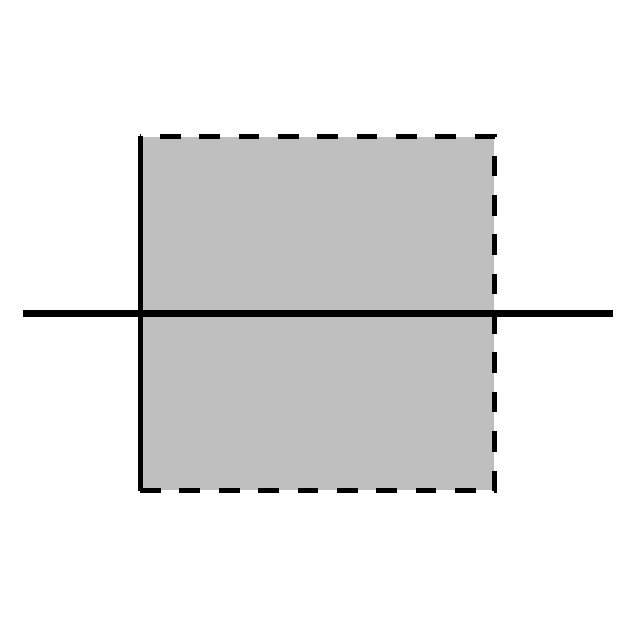
\includegraphics[height=\fsize]{figs/ex_16_8_1} &
    \text{(b)} &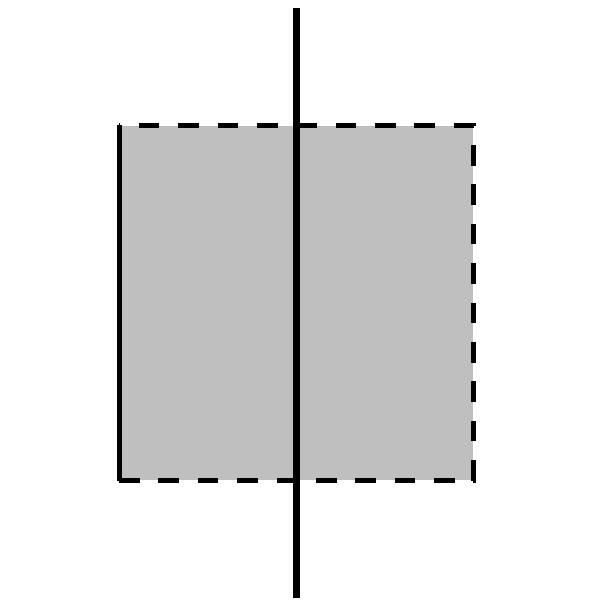
\includegraphics[height=\fsize]{figs/ex_16_8_2} &
    \text{(c)} &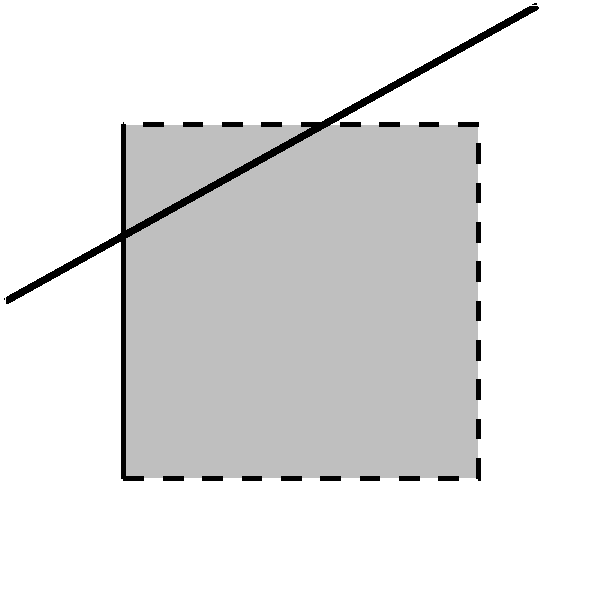
\includegraphics[height=\fsize]{figs/ex_16_8_3} \\
    \text{(d)} &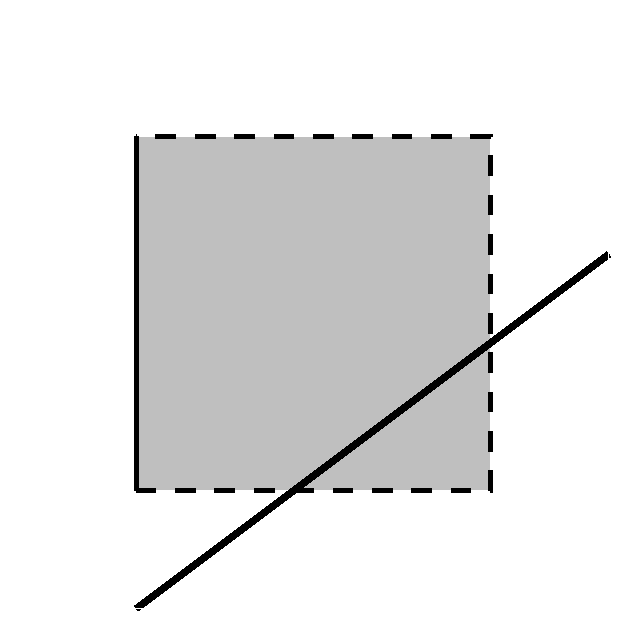
\includegraphics[height=\fsize]{figs/ex_16_8_4} &
    \text{(e)} &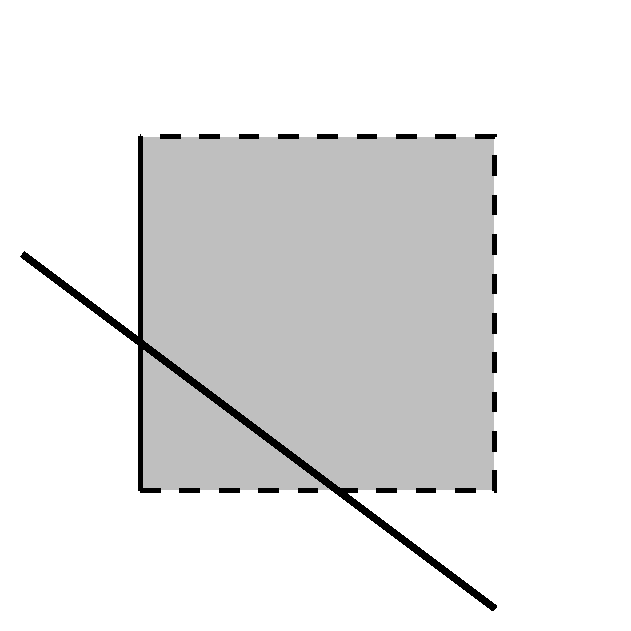
\includegraphics[height=\fsize]{figs/ex_16_8_5} &
    \text{(f)} &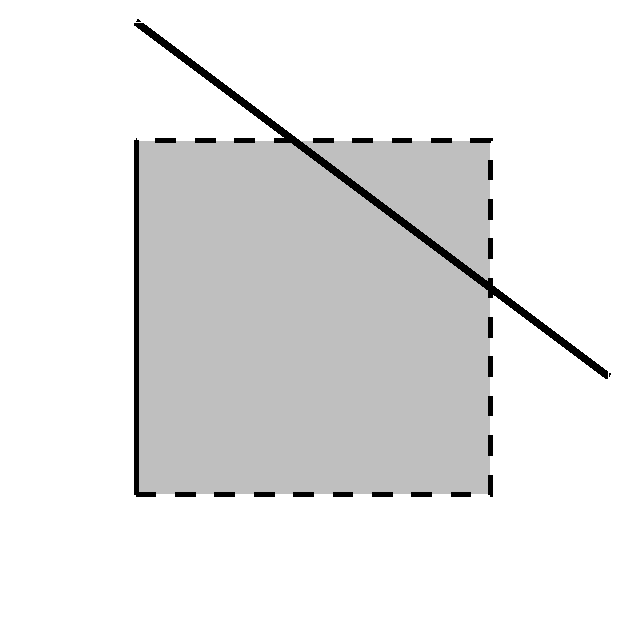
\includegraphics[height=\fsize]{figs/ex_16_8_6}
  }
  Clearly the intersection of $L$ and these basis elements results in some kind of interval on $L$.
  Such intervals then form the basis for the subspace topology on $L$ by Lemma~16.1 since they are the intersection of $L$ and a basis element in the superspace.
  Another point is that the orientation of the line $L$ with regard to the way in which it is a copy of $\reals$ is important.
  For example, in Figure~(a) above, if $L$ is oriented in the natural way with the negative reals on the left and the positive reals on the right, then the resulting intervals are of the form $\clop{a,b}$, which would result in a topology like \Rl.
  The opposite orientation results in intervals of the form $\opcl{a,b}$ as basis elements, generating a topology like \Ru.

  Now, for a line $L$ such as that illustrated in Figure~(a), every possible basis element of $\reals_l \times \reals$ that intersects $L$ results the half-open intervals as described above depending on the orientation of $L$.
  This is not the case for all lines, however, and is dependent on its slope in the plane.
  For example, lines with positive slope can intersect basis elements as in Figure~(c), which result in half open intervals $\clop{a,b}$ (or $\opcl{a,b}$ depending on orientation), or they can intersect them as in Figure~(d), which result in open intervals $(a,b)$.
  However, since the topologies \Rl and \Ru are strictly finer than the standard topology, the subspace topology formed on $L$ would be like these (which depends on orientation) rather than like the standard topology.
  Lastly, we note that, for any appropriate interval on the line $L$, we can clearly always find a basis element $B$ in $\reals_l \times \reals$ such that the intersection of $B$ with $L$ is the interval.
  For this reason, these intervals form the basis elements of the topology on $L$.

  With all these considerations in mind, we list the topologies on $\reals$ that the subspace topologies on $L$ are like based on line directions and orientations for product topologies $\reals_l \times \reals$ and $\reals_l \times \reals_l$:
  \begin{center}
    \begin{tabular}{c|cc}
      $L$ & $\reals_l \times \reals$ & $\reals_l \times \reals_l$ \\
      \hline
      $\rightarrow$ & \Rl & \Rl \\
      $\nearrow$ & \Rl & \Rl \\
      $\uparrow$ & $\reals$ & \Rl \\
      $\nwarrow$ & \Ru & \Rd \\
      $\leftarrow$ & \Ru & \Ru \\
      $\swarrow$ & \Ru & \Ru \\
      $\downarrow$ & $\reals$ & \Ru \\
      $\searrow$ & \Rl & \Rd
    \end{tabular}
  \end{center}
  We note that $\reals$ simply denotes the standard topology.
}
